
\section{Webserver}

\begin{frame}{Webserver}
	\begin{itemize}
		\item Python Server mit Flask API
		\item \begin{itemize}
			\item stellt Endpunkte zum Persistieren der Stammdaten
			\item stellt Endpunkte zur Live Administration einer Übung
			\item stellt Endpunkte zur Teilnahme an einer Übung
		\end{itemize}
		\item React Webframework für Frontend
	\end{itemize}
\end{frame}

\begin{frame}{Webserver}
	\begin{figure}
		\begin{center}
			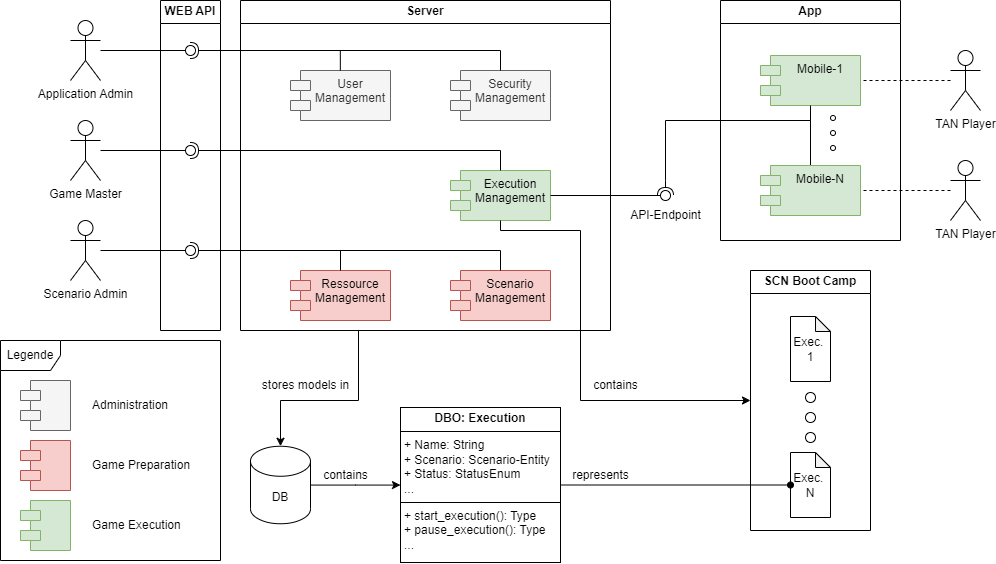
\includegraphics[width=0.7\textwidth]{images/server/component_diagram.png}
		\end{center}
		\caption{Komponentendiagramm Webserver MANVSim}\label{fig:autounfall}
	\end{figure}
\end{frame}
